\section{Graphical User Interfaces of {\twodx}}
\label{sec:gui}
\index{Graphical User Interface}

In this chapter we give an overview of the programs in the {\twodx}-package. We distinguish between {\twodx}\texttt{\_merge} (\autoref{sec:2dx_merge}) for merging multiple density maps generated from individual images by {\twodx}\texttt{\_image} (\autoref{sec:2dx_image}). Additionally we give some details about further technical subtleties in \autoref{sec:tech_details}.

\subsection{{\twodx}\texttt{\_merge} Overview of the Graphical User Interface}
\label{sec:2dx_merge}
\index{Graphical User Interface ! {\twodx}\textit{\_merge}}
\autoref{fig:gui_overview_merge} shows the {\twodx}\texttt{\_merge} graphical user interface, which will be discussed in the following section. The present interface is the starting point for each {\twodx}-project as all the micrographs are managed and finally merged here.

\begin{figure}[H]
	\centering
	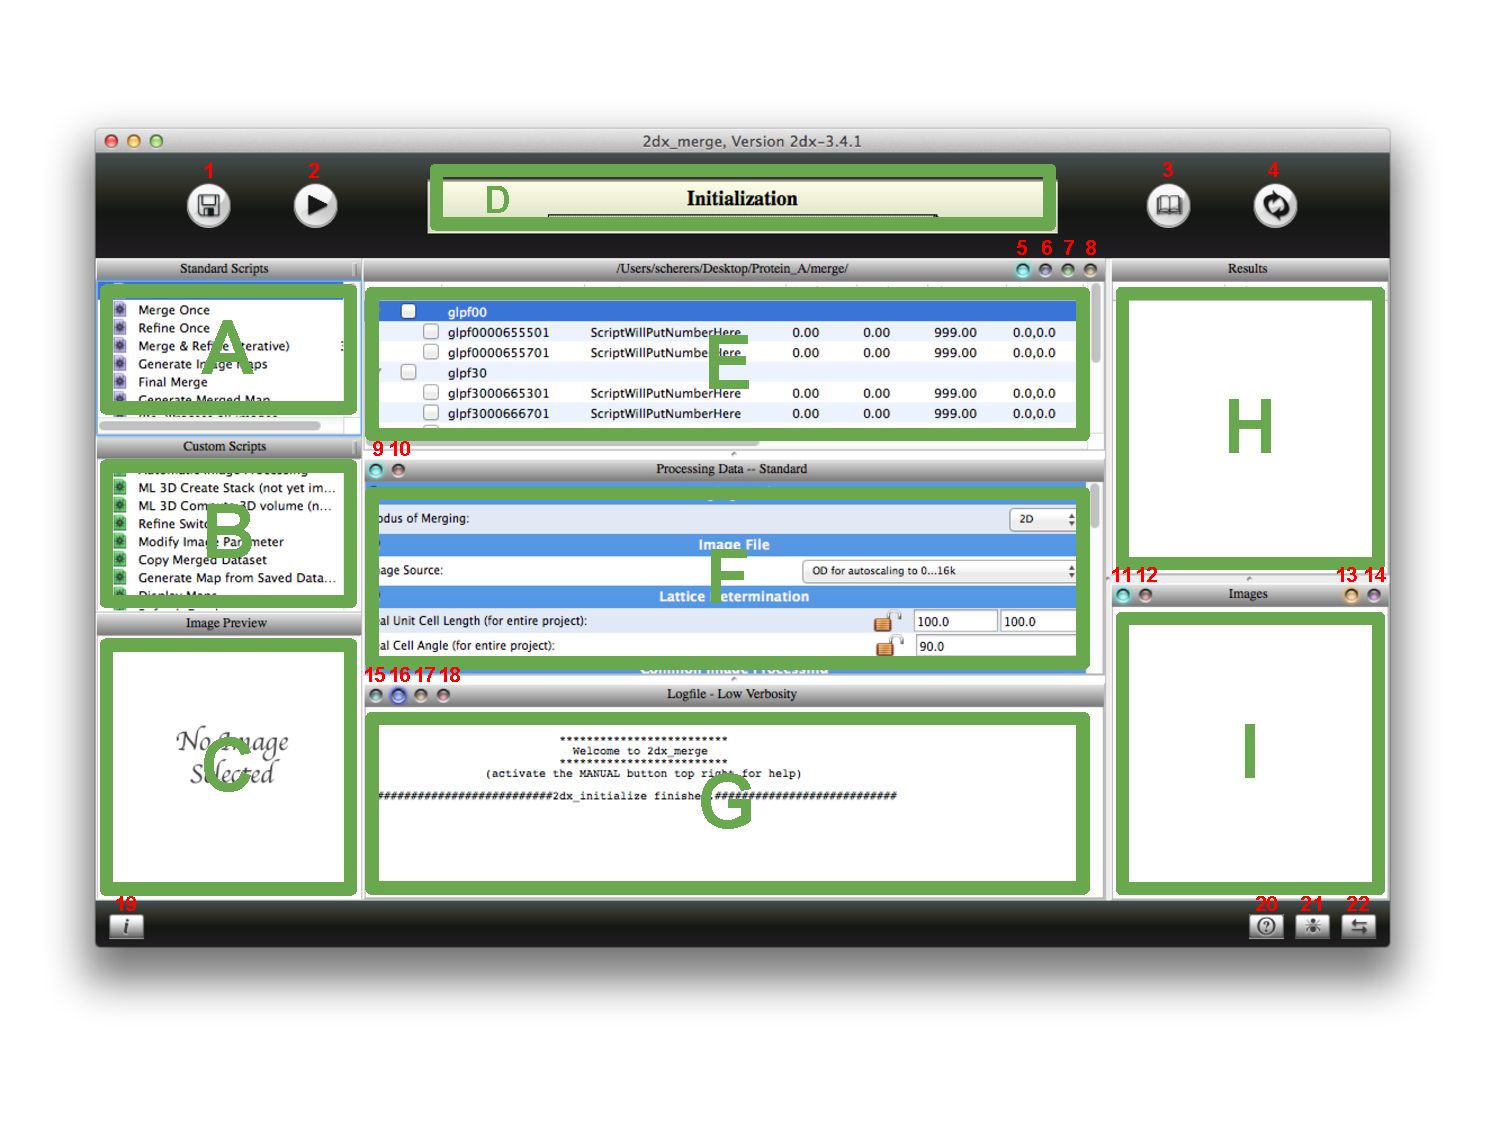
\includegraphics[width=.99\textwidth]{gui_overview.pdf}
	\caption{{\twodx}\texttt{\_merge} graphical user interface}
	\label{fig:gui_overview_merge}
\end{figure}

In the following we distinguish between panel (green boxes) and buttons (red numbers). {\twodx}\texttt{\_merge} consists of the following panel:


\begin{description}
	\item[A - Standard Scripts] All standard processing scripts are grouped in this panel. You can select one or multiple scripts by clicking on them. A double-click will open the script in a text editor and allows you to change the script to your needs. Note that it may be that you have to configure which text editor is opened before you open the first script. The corresponding manual can be found in \autoref{sec:open_program}.
	\item[B - Custom Scripts] Similar to the \textit{Standard Scripts}, but these scripts usually are not needed for simple processing but may be useful for non standard tasks or managing your project.
	\item[C - Image Preview] Once you selected an image in panel \textit{I - Image Preview Panel} you can either see the header of the selected image or a preview.
	\item[D - Status Bar] The status bar shows the progress of the running script. Note that only approximate value are shown.
	\item[E - Project Panel] All micrographs of your current project are collected in this panel. The micrographs are grouped by their name and tilt angle into folders. You can select individual micrographs by clicking the checkbox in front of the image name. You can also select an entire tilt series by selecting the corresponding top-level directory. In \autoref{sec:project_panel} we explain how you can customize this panel.
	\item[F - Parameter Panel] Once you selected a script from panel A or B all the corresponding parameters show up in this panel. On the left side the parameter name is shown and its value can be set on the right side. Clicking on a parameter name with the right mouse button opens a help window where you get a short summary of the parameter. Some of the parameters can be locked (by clicking on the lock) in order to prevent them from being overwritten accidentally. Note that you can change the verbosity level of the parameter panel with the buttons 9 to 10. 
	\item[G - Log Panel] All our scripts generate some terminal output which is shown in this panel. Note that you can change the verbosity level of the log panel with the buttons 15 to 19.  
	\item[H - Results Panel] During the calculations some scripts generate resulting values, which might be important to know for experienced users. All these values are listed in the present panel.
	\item[I - Image Panel] Some of the scripts generate some resulting images or files which are listed in this panel. For example you will find the finally merged map in this panel.
\end{description}

Beside the panels mentioned above {\twodx}\texttt{\_merge} has a bunch of buttons which allow the user to launch calculations or change the look if the graphical user interface:

\begin{description}
	\item[1 - Save Configuration] Saves the current parameter set to the configuration file
	\item[2 - Launch Script] Launches the script or scripts selected either in \textit{Standard Scripts} or \textit{Custom Scripts}.
	\item[3 - Show/Hide Manual] This button shows you the quick reference of the selected script. The manual can be hidden again by clicking on the button once more.
	\item[4 - Refresh Results] Force {\twodx} to reload all generated results.
	\item[5 - Default View] Change to view back to the default setting.
	\item[6 - Maximize Project Panel] Maximizes the \textit{Project Panel} while removing all the panels E-H from the current view.
	\item[7 - Maximize Parameter Panel] Similar to \textit{Maximize Project Panel} but this button maximizes the parameter panel at the other's panel presence.
	\item[8 - Maximize Log Panel] Maximizes the \textit{Log Panel}.
	\item[9 - Show Simple Parameters] {\twodx} support two parameter setting modes. With this button you can change to the simple parameter mode.
	\item[10 - Show Advanced Parameters] The expert parameter mode can be activated by means of this button.
	\item[11 - Show All Images] {\twodx} distinguishes between all and important images generated by the launched scripts. The mode activated by this button shows you all generated images.
	\item[12 - Show Important Images] The present button only shows you the important generated images
	\item[13 - Show Nicknames] The names of the generated images can be shown in two different modes. Either you can use nicknames which describe in a compact fashion what kind of information the image contains or you can use the original filename. The nickname mode is activated by pressing this button
	\item[14 - Show Full Filenames] In order to see the original filename of the generated images click on this button.
	\item[15 - Silent Log Mode] {\twodx}'s log output can be generated in different verbosity levels. You can select the level of your needs with the button $15$ to $18$. In this \textit{Log Panel} mode only the script terminations are reported.
	\item[16 - Low Log Mode] Shows all the important information generated by the scripts.
	\item[17 - Moderate Log Mode] Gives you some additional output compared to the low verbosity.
	\item[18 - Highest Log Mode] Shows you all output generated by the scripts. Note this mode may slow down the execution of the script.
	\item[19 - Show/Hide Preview] \textit{Image Preview} can either show the header of the selected file or a preview of the context. This button allows you to change between the two modes.
	\item[20 - View Online Help] Redirects you to our online help
	\item[21 - Launch Bug Tracker] Redirect you to the {\twodx} bug tracker. You are kindly requested to report all observed issues.
	\item[22 - Stop Sync with Config] Change to the "Dry Run" mode to test the execution of a script without potentially messing up your configuration file. Don't forget to change the mode back in case you want to overwrite the current configuration.
\end{description}



\subsection{Additional Technical Aspects for {\twodx}\texttt{\_merge}}
\label{sec:tech_details}
In this section we discuss additional technical aspects such as customizing the project panel, the structure of a {\twodx}-project and regular expressions. The deep understanding of these additional tricks in general is not absolutely required for successfully processing your images.

\subsubsection{Customizing the Project Panel}
\label{sec:project_panel}
\index{Project Panel}

During processing the individual images with {\twodx}\texttt{\_image} a lot of different parameters are calculated for each images. These parameters can be displayed in {\twodx}\texttt{\_merge}'s \textit{Project Panel}. The default parameter selection can be adapted to your needs by simply right-clicking on the parameter header. You can choice your parameter selection in the appearing selection list as shown in \autoref{fig:project_panel_params}.

\begin{figure}[H]
	\centering
	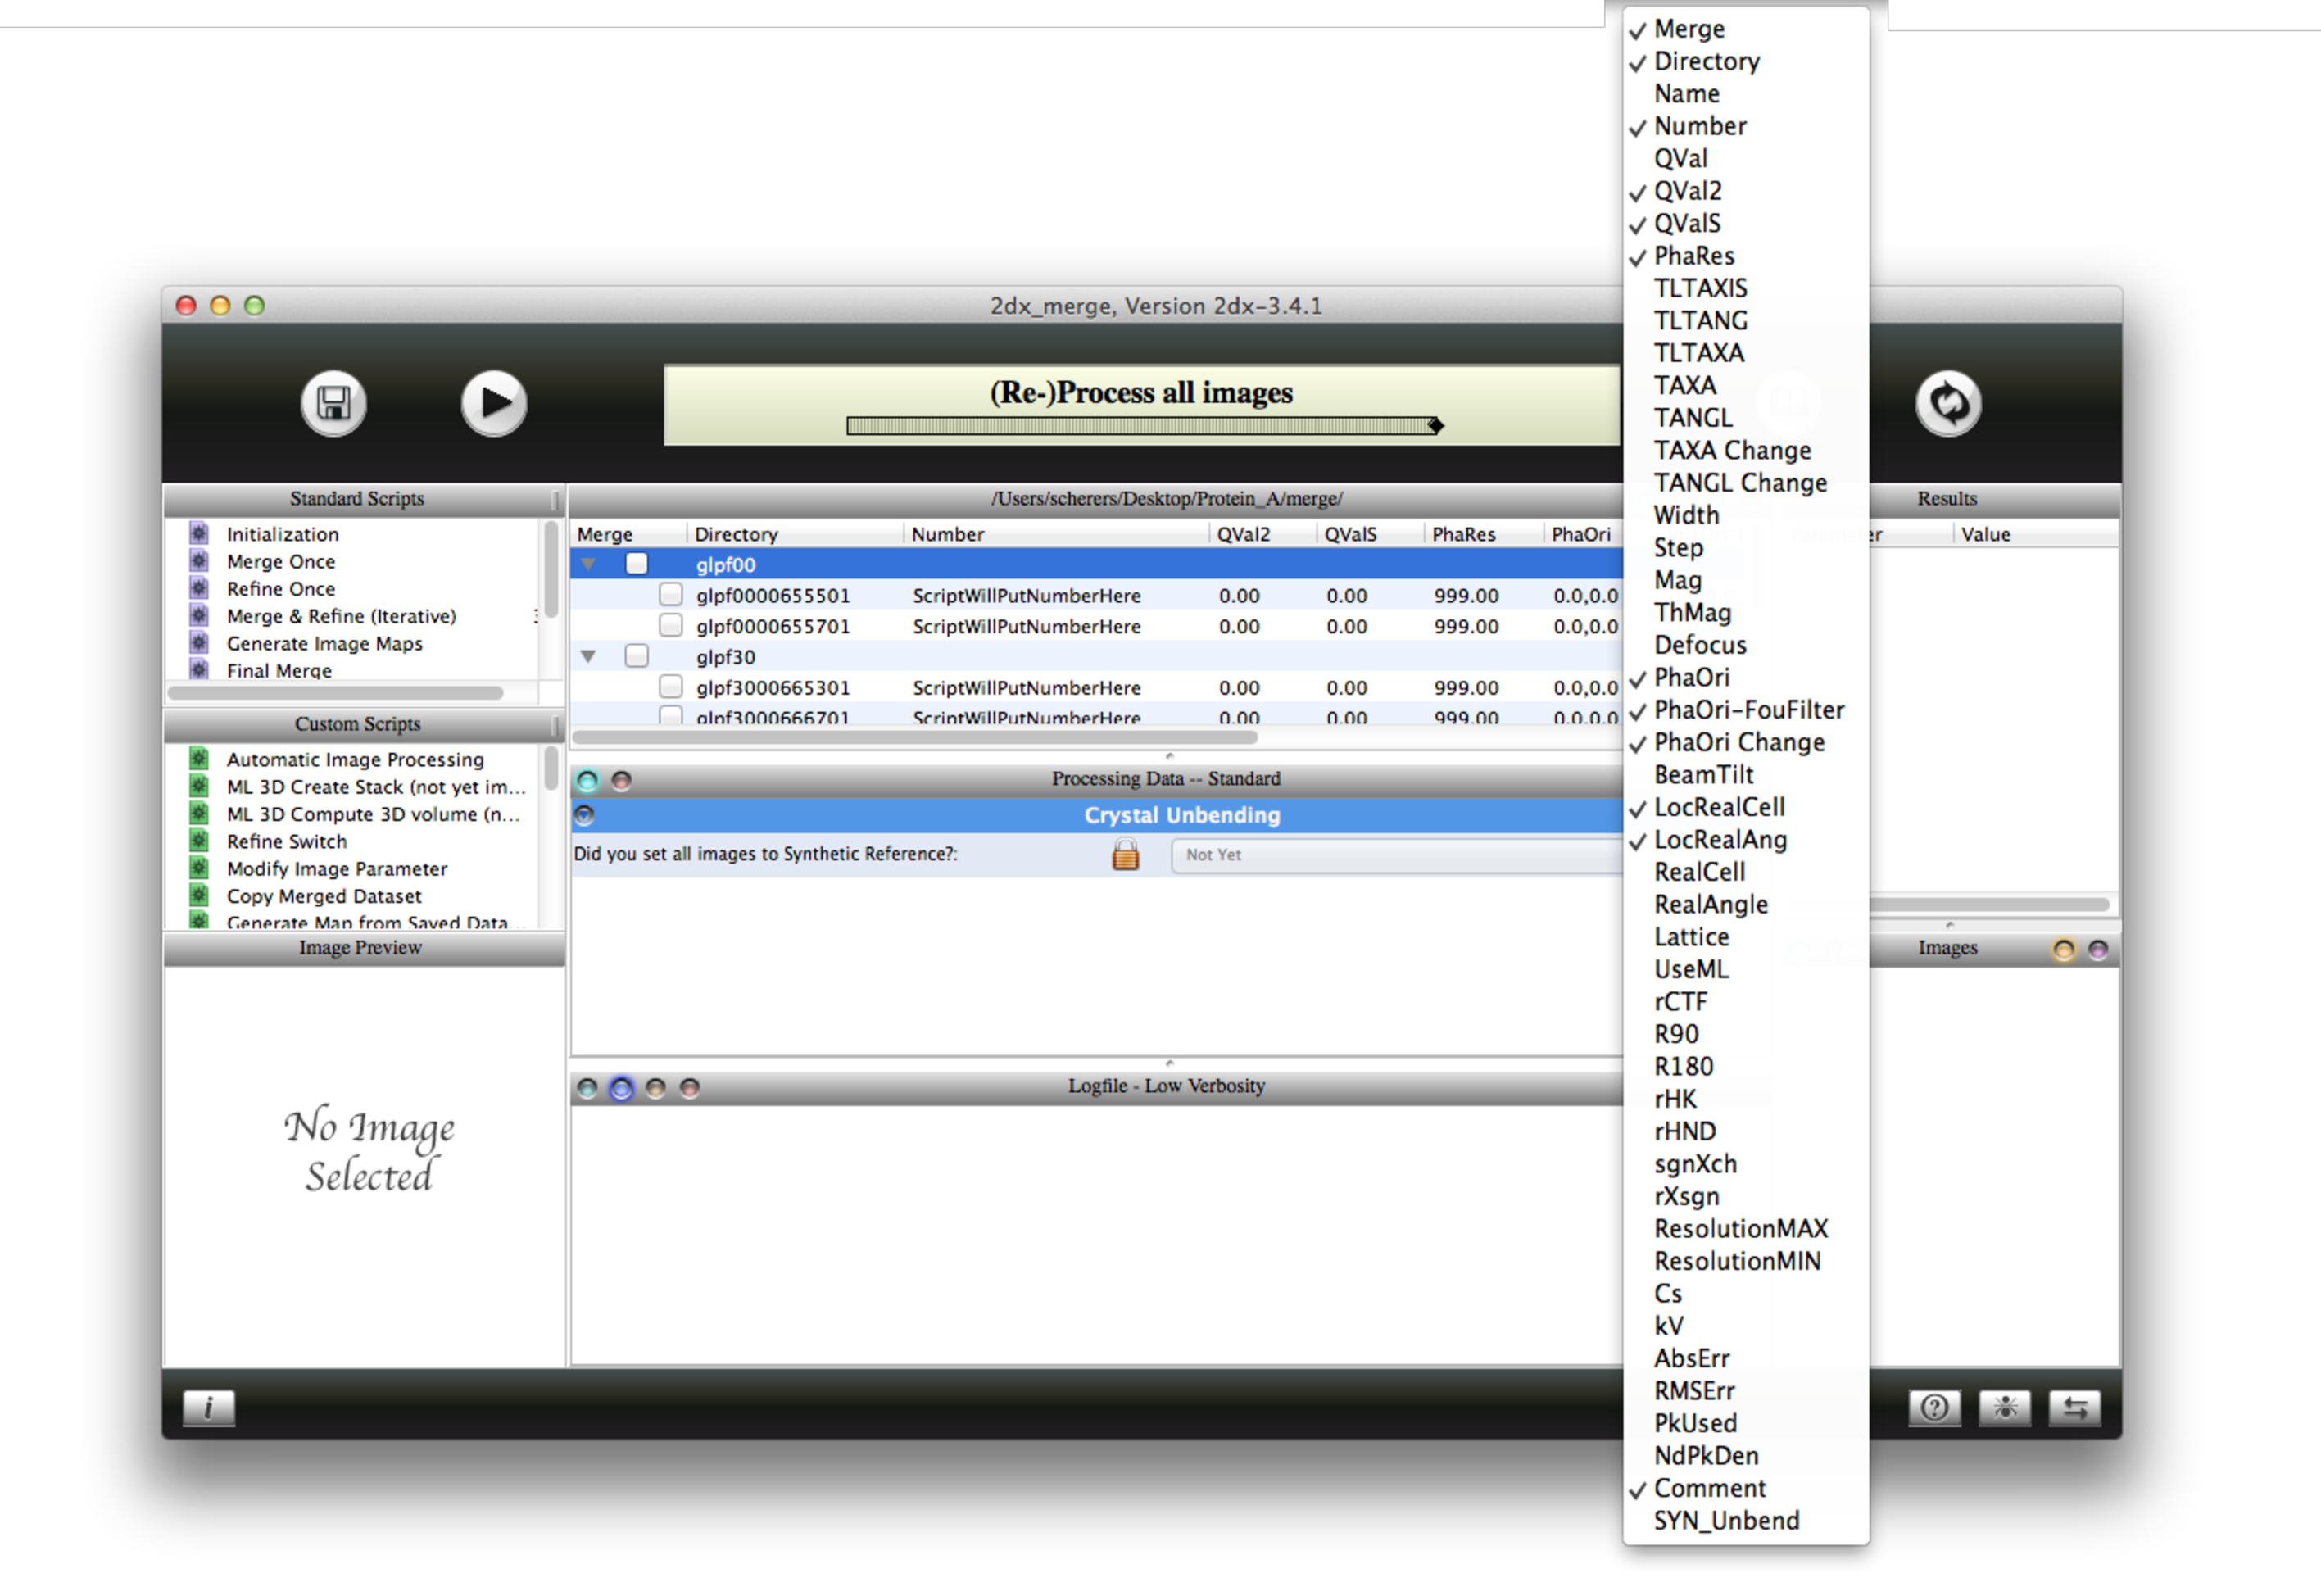
\includegraphics[width=.99\textwidth]{merge_change.pdf}
	\caption{Change the shown parameters of the project panel}
	\label{fig:project_panel_params}
\end{figure}


\subsubsection{Customizing Third-Party Program Calls}
\index{Program Preferences}
\label{sec:open_program}

Some of the file generated by {\twodx} can not be open natively in {\twodx}, e.g. \textit{.pdf} or 3D volumes. Double-clicking on these files the \textit{Images Panel} opens a third-party program installed on your machine. The corresponding setting can be adapted under "2dx\_merge > Preferences" as shown in \autoref{fig:merge_prefs}. In order to change the settings please enter the corresponding command which launches the desired third-party application in the terminal. Dependent on your operating system we use different default values, but dependent on the installed software you probably have to configure the setting.

\begin{figure}[H]
	\centering
	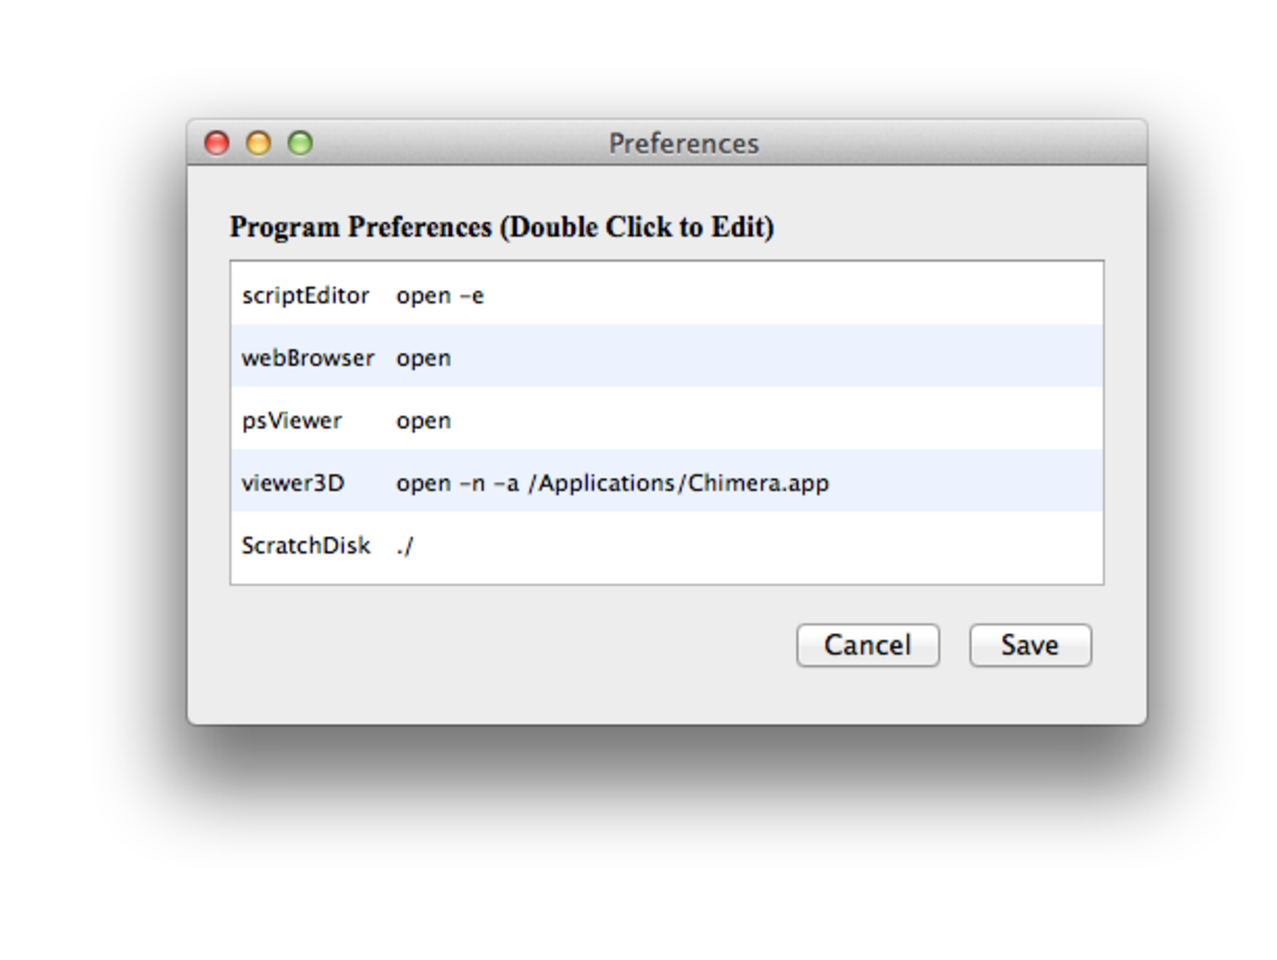
\includegraphics[width=.85\textwidth]{merge_prefs.pdf}
	\caption{Program Preferences}
	\label{fig:merge_prefs}
\end{figure}


\subsubsection{{\twodx} Project Structure}
\index{Project structure}
\label{sec:project_struc}

A {\twodx}-project directory contains the following folder and files:

\begin{itemize}
	\item \textbf{2dx\_master.cfg} is the top-level configuration file which serves as default configuration files for all calculations performed on the entire project. Note that you should not edit these files manually as they are usually set trough the graphical user interface.
	\item \textbf{merge-folder} contains all the files generated while merge multiple images by means of {\twodx}\texttt{\_merge}.
	\item \textbf{Folders per tilt angle:} {\twodx} generates a folder for each tilt angle. Each image and all the corresponding files generated during the single image processing are stored in an individual folder in the corresponding tilt angle folder. 
\end{itemize}


\subsubsection{Regular Expressions}
\index{Regular expression}
\label{sec:regexp}

One of the imported micrographs was called \textit{glpf0000655301.tif}. The additional information was parsed by the following regular expression (\autoref{sec:import}): \texttt{\^{}(\textbackslash w\{4\})(\textbackslash d\{2\})(\textbackslash d\{6\})(\textbackslash d\{2\})\$}. The $4$ after the "w" defines the number of letters used for the protein name. The next block tells that two digits are used to store the tilt angle. Analogously the image number consists of $6$ digits respectively the sub-image number of two digits. If you want to use another convention you have to change the number of digits of the additional information fields. Note that the total amount of used letters should equal the number of letters used for the entire filename. Once you defined the regular expression of your needs you can store the expression by clicking on the "+"-button.

{\twodx} comes with a set of different predefined regular expressions from which you can choice or which you also can edit. For instance the following expression allows underscores between the different information fields: \texttt{\^{}(\textbackslash w\{4\}).*\_(\textbackslash d\{2\}).*\_(\textbackslash d\{6\}).*\_(\textbackslash d\{2\})\$}.

\subsubsection{The \texttt{\textasciitilde /.2dx} folder}
{\twodx} generates a hidden folder \texttt{\textasciitilde /.2dx} in your home directory. In this folder we store some global configurations for {\twodx}, such as your personal regular expressions or third party application configurations. Please to not change the content of the folder manually. In case you want to reset all your settings you can simple remove this folder.


\newpage
\subsection{{\twodx}\texttt{\_image} Overview of the Graphical User Interface}
\label{sec:2dx_image}
\index{Graphical User Interface ! {\twodx}\textit{\_image}}

Single micrographs are processed by means of {\twodx}\texttt{\_image}. Double-clicking a filename in the {\twodx}\texttt{\_merge}'s \textit{Project Panel} launches {\twodx}\texttt{\_image} for the corresponding micrograph. Note that before you can merge the images you have to process them in {\twodx}\texttt{\_image} through the graphical user interface shown in \autoref{fig:gui_overview_image} and explained in the following. A bunch of panels and buttons have the same functionality as in {\twodx}\texttt{\_merge} therefore these points are not discussed in details here and you are asked to lookup the description in \autoref{sec:2dx_merge}.

\begin{figure}[H]
	\centering
	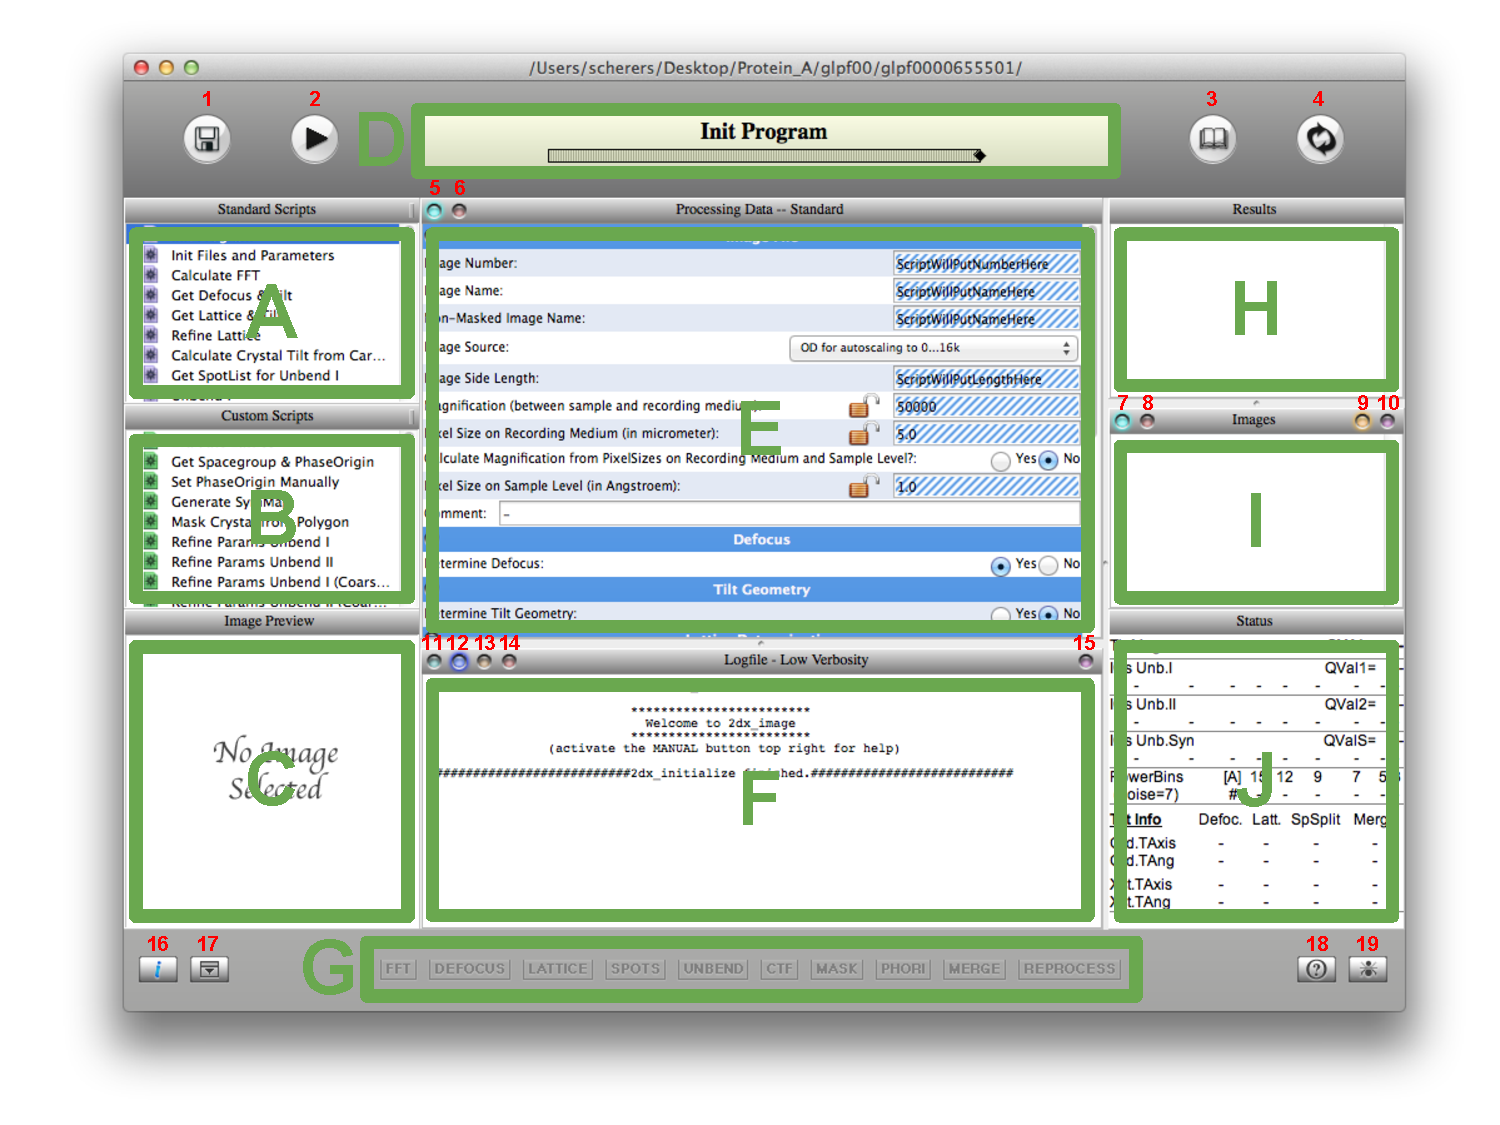
\includegraphics[width=.99\textwidth]{image_overview.pdf}
	\caption{{\twodx}\texttt{\_image} graphical user interface}
	\label{fig:gui_overview_image}
\end{figure}

\begin{description}
	\item[A - Standard Scripts] Scripts for standard single image processing. If you select and launch all the scripts you get the first approximate two-dimensional map from your crystal.
	\item[B - Custom Scripts] More advanced single image processing scripts
	\item[C - Image Preview] Preview of the resulting images
	\item[D - Process Bar] Tells you which script is running and show the actual progress.
	\item[E - Parameter Panel] Panel meant for changing the parameters of the selected script
	\item[F - Log Panel] Log output is shown here.
	\item[G - Stamps Panel] Once a processing step is done the corresponding box gets darker. After successfully processing an image all boxes should be dark. This panel helps you to not forget one of the processing steps.
	\item[H - Results Panel] Results generated by the scripts are listed in this panel.
	\item[I - Images Panel] Intermediate images are collected here.
	\item[J - Status Panel] {\twodx} calculates automatically a bunch of values which indicate the quality of the actual processing result. In order to have these values always at hand they are collected in this panel.
\end{description}


\begin{description}
	\item[1 - Save Config] Save the config file to disk.
	\item[2 - Launch Script] Launch the selected script(s).
	\item[3 - Show/Hide Manual] Open or closes the manual view of the selected script
	\item[4 - Refresh Results] Reload the \textit{Result Panel}.
	\item[5 - Show Simple Parameters] Shows the simple parameter interface of the selected script.
	\item[6 - Show Advanced Parameters] Shows the advanced parameter interface of the selected script.
	\item[7 - Show All Images] Shows all generated images in the \textit{Images Panel}.
	\item[8 - Show Important Images] Shows only the important generated images in the \textit{Images Panel}.
	\item[9 - Show Nicknames] Shows the nicknames of the generated images in the \textit{Images Panel}.
	\item[10 - Show Full Filenames] Shows the full filename of the generated images in the \textit{Images Panel}.
	\item[11 - Silent Log Mode] Switches the \textit{Log Panel} to silent mode.
	\item[12 - Low Log Mode] Switches the \textit{Log Panel} to low verbosity mode.
	\item[13 - Moderate Log Mode] Switches the \textit{Log Panel} to moderate verbosity mode.
	\item[14 - Highest Log Mode] Switches the \textit{Log Panel} to high verbosity mode.
	\item[15 - Show Processing History] In {\twodx}\texttt{\_image} you can switch between reading the log and the history of you calculations. The log just shows you the current output of the scripts, but the history browser shows you some parameters and results from previous runs. This feature can be used to optimize certain processing parameters in order to lookup previous quality measures gained by different parameter settings.
	\item[16 - Switch Header-Preview] Changes between header and preview of the generated image selected from \textit{Images Panel}.
	\item[17 - Show/Hide Preview] Shows or Hide the \textit{Image Preview}.
	\item[18 - View Online Help] Opens online help.
	\item[19 - Launch Bug Tracker] Opens the online bug tracker.
\end{description}

\newpage
\subsection{{\twodx}\texttt{\_logbrowser}}
\index{Graphical User Interface ! {\twodx}\textit{\_logbrowser}}
{\twodx} generates a bunch of log output during the calculations. Additionally the output is generated in different verbosity levels as explained in \autoref{sec:2dx_merge}. The {\twodx}\texttt{\_logbrowser} allows you to have a look at the log output in a more human readable way as shown in \autoref{fig:gui_overview_log}. 

\begin{figure}[H]
	\centering
	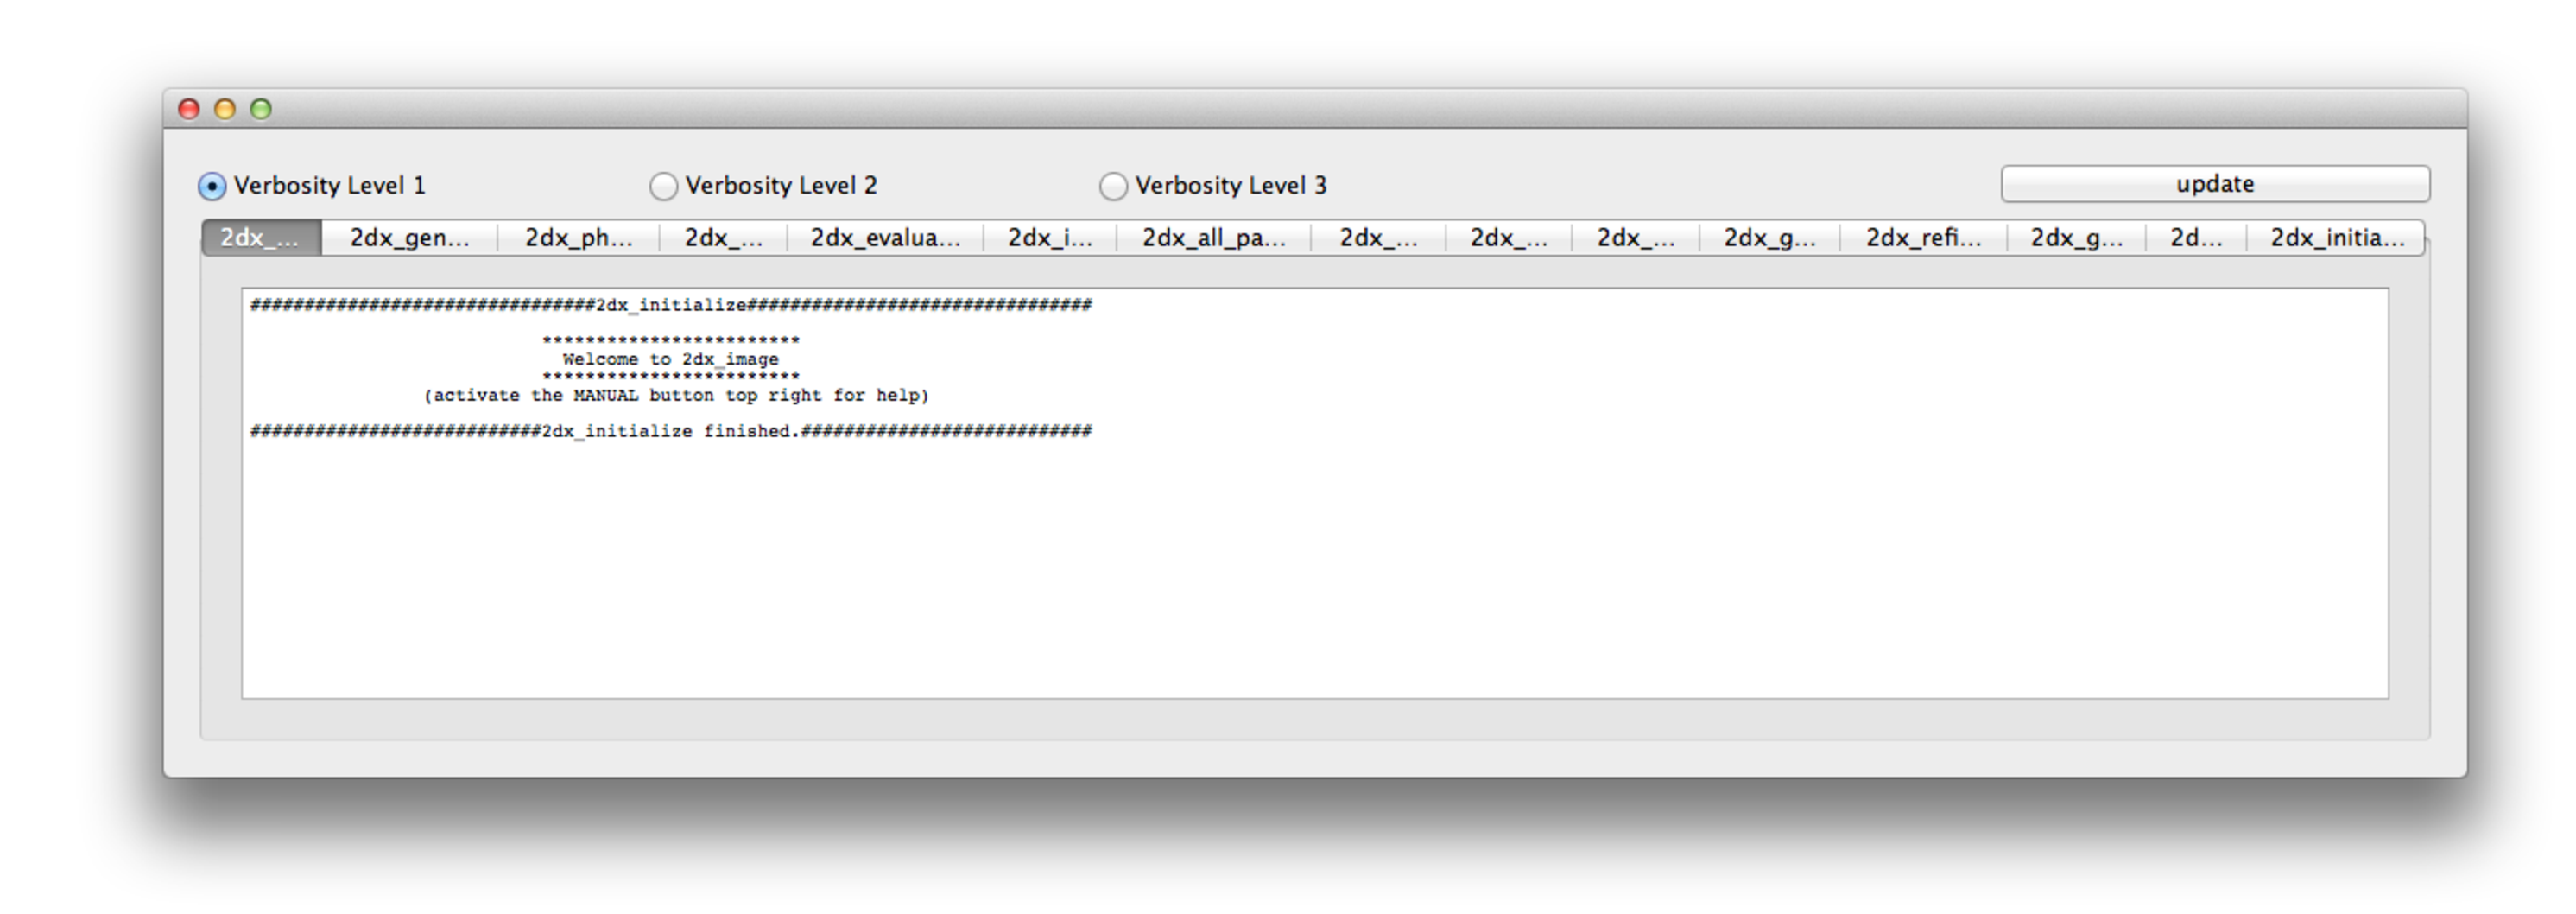
\includegraphics[width=.99\textwidth]{gui_log.pdf}
	\caption{{\twodx}\texttt{\_logbrowser} graphical user interface}
	\label{fig:gui_overview_log}
\end{figure}

You can open the {\twodx}\texttt{\_logbrowser} by double-clicking on the header of the Log Panel in {\twodx}{\_merge} or {\twodx}\texttt{\_image}.

The graphical user interface of the {\twodx}\texttt{\_logbrowser} should be self-explanatory in general. You can change the verbosity level of the shown log output be clicking on the corresponding verbosity check box. Above the panel in which the log is finally presented you can select from which program you want to see the log. The "update" button reloads the shown log file in order to display also the latest changes.